% 2018 上海卷第15题：正六棱柱与阳马
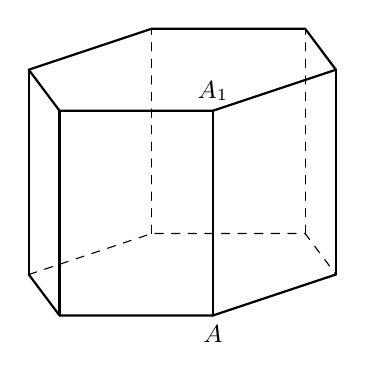
\begin{tikzpicture}[font=\small, line cap=round, line join=round, >=stealth, scale=1.3]
  % 顶面顶点坐标（以仿射投影正六边形建模，对边平行且相等）
  \coordinate (A1) at (0.3, 1.8);
  \coordinate (L1) at (-1.2, 1.8);
  \coordinate (L2) at (-1.5, 2.2);
  \coordinate (T1) at (-0.3, 2.6);
  \coordinate (T2) at (1.2, 2.6);
  \coordinate (R1) at (1.5, 2.2);

  % 底面顶点坐标（垂直向下平移 2.0）
  \coordinate (A)  at (0.3, -0.2);
  \coordinate (BL1) at (-1.2, -0.2);
  \coordinate (BL2) at (-1.5, 0.2);
  \coordinate (BT1) at (-0.3, 0.6);
  \coordinate (BT2) at (1.2, 0.6);
  \coordinate (BR1) at (1.5, 0.2);

  % 隐藏棱（虚线）
  \draw[dashed, thin] (BT1) -- (T1);
  \draw[dashed, thin] (BT2) -- (T2);
  \draw[dashed, thin] (BL2) -- (BT1) -- (BT2) -- (BR1);

  % 可见侧棱与底面棱（实线）
  \draw[thick] (BL2) -- (L2);
  \draw[thick] (BL1) -- (L1);
  \draw[thick] (A)   -- (A1);
  \draw[thick] (BR1) -- (R1);
  \draw[thick] (BL2) -- (BL1) -- (A) -- (BR1);

  % 顶面棱（全部可见，实线）
  \draw[thick] (L1) -- (A1) -- (R1) -- (T2) -- (T1) -- (L2) -- cycle;

  % 顶点标签
  \node[above] at (A1) {$A_1$};
  \node[below] at (A)  {$A$};
\end{tikzpicture}
